%! Author = Krzysztof Pietruczuk GR2 - Matematyka Ist. semestr 1
%! numer albumu: 97421
%! Date = 19.10.2024

% Preamble
% Zdefiniowanie klasy dokumentu
\documentclass[12pt, a4paper]{report}

% Packages
\usepackage{amsfonts}
\usepackage{amssymb}


% Dołączanie potrzebnych pakietów

\usepackage[polish]{babel}     % Ustawienie języka polskiego
\usepackage[utf8]{inputenc}    % Obsługa polskich znaków UTF-8
\usepackage[T1]{fontenc}       % Właściwe kodowanie fontów dla polskich znaków
\usepackage{adjustbox}
\usepackage{graphicx}
\usepackage{changepage}
\usepackage{fancyhdr}
\usepackage[left=2cm,right=1.5cm,top=2cm,bottom=2cm]{geometry}
\usepackage{setspace}
\usepackage{enumitem}
\usepackage{amsmath}
\usepackage{multirow}
\usepackage{color}


%definicje wlasnych komend
\DeclareMathOperator{\Q}{\mathbb{Q}}
\DeclareMathOperator{\R}{\mathbb{R}}
\DeclareMathOperator{\Z}{\mathbb{Z}}
\DeclareMathOperator{\N}{\mathbb{N}}
\DeclareMathOperator{\C}{\mathbb{C}}

%srodowiska
\newtheorem{prz}{Przykład}

% Document
\begin{document}

    \begin{center}
        \textbf{Krzysztof Pietruczuk, grupa 2}

        \textbf{nr albumu: 97421}
    \end{center}

    \medskip

    \noindent
    \textbf{Zadanie 4.7}

    \noindent
    Rozwiązać równanie $2 \leq |4 - x| < 7$

    \bigskip
    \noindent
    \emph{\textbf{Rozwiązanie}}


    \noindent
    Dziedziną nierówności $2 \leq |4 - x| < 7$ jest cały zbiór $\R$, czyli wszystkie liczby rzeczywiste.
    Nierówność nie zawiera żadnych operacji, które ograniczałyby dziedzinę. Wartość bezwzględna $|4 - x|$
    jest dobrze zdefiniowana dla wszystkich $\R$.

    \medskip

    \noindent
    Rozpatrywana nierówność jest zapisana w formie złożonej, w której kilka warunków dotyczących jednej zmiennej
    jest zapisanych w jednym wyrażeniu równocześnie, dlatego należy rozpatrzyć dwa warunki dla wartości bezwzględnej w tej nierówności:
    \[
        \begin{cases}
            |4 - x| \geq 2 \\
            |4 - x| < 7
        \end{cases}
    \]

    \vspace{20pt}                            % dodaje 20 punktów odstępu w pionie

    \noindent
    \textbf{Etap 1}

    \noindent
    Rozwiązanie nierówności $2 \leq |4 - x| < 7$ rozpoczynamy od przypomnienia definicji wartości bezwzględnej która mówi,
    że dla wartości bezwzględnej $|a|$ otrzymujemy:
    \[
        |a| = \begin{cases}
                  a, & \text{gdy } a \geq 0, \\
                  -a, & \text{gdy } a < 0.
        \end{cases}
    \]

    \noindent
    W naszej nierówności odpowiednikiem $a$ z definicji jest $4-x$,
    dlatego dla wartości wyrażenia $|4-x|$ mamy:
    \[
        |4-x| = \begin{cases}
                  4-x, & \text{gdy } 4-x \geq 0, \\
                  -4+x, & \text{gdy } 4-x < 0.
        \end{cases}
    \]
    stąd uzyskujemy:

    \begin{center}                           % Wyśrodkowanie całego bloku poziomo
    \begin{minipage}[c]{0.3\textwidth}       % [c] ustawia wyśrodkowanie pionowe
    \vspace*{\fill}                          % Rozpoczynamy wyśrodkowanie pionowe
    \[
        |4-x| = \begin{cases}
                    4-x, & \text{gdy } x \leq 4, \\
                    -4+x, & \text{gdy } x > 4.
        \end{cases}
    \]
    \vspace*{\fill}                          % Kończymy wyśrodkowanie pionowe
    \end{minipage}
    \hspace{0.05cm}                          % Mały odstęp między kolumnami
    \begin{minipage}[c]{0.4\textwidth}       % [c] ustawia wyśrodkowanie pionowe
        \centering
        \hspace{0.3cm}                       % Przesunięcie obrazka w prawo
        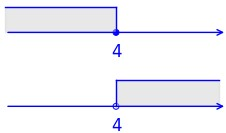
\includegraphics[width=0.55\textwidth]{fig_1.jpg}   % Ustawienie rozmiaru obrazka
        \vspace*{\fill}                      % Wyśrodkowanie pionowe
    \end{minipage}
    \end{center}

    \vspace{20pt}                            % dodaje 20 punktów odstępu w pionie

    \noindent
    \textbf{Etap 2}
    \emph{ - analiza pierwszego warunku dla wartości bezwzględnej $|4-x|$ gdy $|4 - x| \geq 2$}

    \noindent
    Rozwiązujemy dwa przypadki pierwszego warunku (dla $x \leq 4$ oraz $x > 4$):

    \noindent
    \begin{center}
    \begin{minipage}{0.2\textwidth}
        \begin{align*}
            4 - x &\geq 2 \\
            -x &\geq 2 - 4 \\
            -x &\geq -2 \\
            x &\leq 2
        \end{align*}
    \end{minipage}
    \hspace{0.05\textwidth}
    \begin{minipage}{0.04\textwidth}
        \[
        \vee
        \]
    \end{minipage}
    \hspace{0.05\textwidth}
    \begin{minipage}{0.2\textwidth}
        \begin{align*}
        -4 + x &\geq 2 \\
        x &\geq 2 + 4 \\
        x &\geq 6
        \end{align*}
    \end{minipage}
    \end{center}


    \begin{center}
        \begin{minipage}{0.3\textwidth}
            \centering
            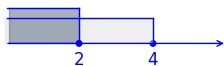
\includegraphics[width=0.6\textwidth]{fig_2.jpg}
            \[x \in (-\infty, 2]\]
        \end{minipage}
        \hspace{0.01\textwidth}
        \begin{minipage}{0.01\textwidth}
        \end{minipage}
        \hspace{0.1\textwidth}
        \begin{minipage}{0.3\textwidth}
            \centering
            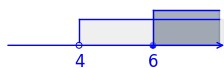
\includegraphics[width=0.6\textwidth]{fig_3.jpg}
            \[x \in [6, +\infty)\]
        \end{minipage}
    \end{center}

    \noindent
    Ostatecznie otrzymujemy jako rozwiązanie $|4 - x| \geq 2$, że $x \in (-\infty, 2] \cup [6, +\infty)$

    \begin{center}
        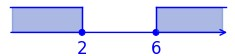
\includegraphics[width=0.22\textwidth]{fig_4.jpg}
    \end{center}

    \vspace{15pt}                            % dodaje 15 punktów odstępu w pionie

    \noindent
    \textbf{Etap 3}
    \emph{ - analiza drugiego warunku dla wartości bezwzględnej $|4-x|$ czyli $|4 - x| < 7$}

    \noindent
    Rozwiązujemy dwa przypadki drugiego warunku (dla $x \leq 4$ oraz $x > 4$):

    \noindent

    \noindent
    \begin{center}
        \begin{minipage}{0.2\textwidth}
            \begin{align*}
                4 - x &< 7 \\
                -x &< 7 - 4 \\
                -x &< 3 \\
                x &> -3
            \end{align*}
        \end{minipage}
        \hspace{0.05\textwidth}
        \begin{minipage}{0.04\textwidth}
            \[
                \vee
            \]
        \end{minipage}
        \hspace{0.05\textwidth}
        \begin{minipage}{0.2\textwidth}
            \begin{align*}
                -4 + x &< 7 \\
                x &< 7 + 4 \\
                x &< 11
            \end{align*}
        \end{minipage}
    \end{center}


    \begin{center}
        \begin{minipage}{0.3\textwidth}
            \centering
            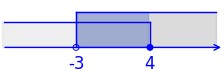
\includegraphics[width=0.6\textwidth]{fig_5.jpg}
            \[x \in (-3,4]\]
        \end{minipage}
        \hspace{0.01\textwidth}
        \begin{minipage}{0.01\textwidth}
        \end{minipage}
        \hspace{0.1\textwidth}
        \begin{minipage}{0.3\textwidth}
            \centering
            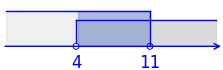
\includegraphics[width=0.6\textwidth]{fig_6.jpg}
            \[x \in (4, 11)\]
        \end{minipage}
    \end{center}

    \bigskip

    \noindent
    Ostatecznie otrzymujemy jako rozwiązanie $|4 - x| < 7$, przedział $x \in (-3, 11)$

    \begin{center}
        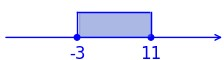
\includegraphics[width=0.2\textwidth]{fig_7.jpg}
    \end{center}

    \vspace{15pt}                            % dodaje 15 punktów odstępu w pionie

    \noindent
    \textbf{Etap 4}
    \emph{ - wyznaczenie części współnej dla obu warunków nierówności $2 \leq |4 - x| < 7$}

    \noindent
    W celu wyznaczenia części wspólnej obu warunków nierówności $2 \leq |4 - x| < 7$ nanosimy na oś liczbową przedziały otrzymane z rozwiązań nierówności $|4 - x| \geq 2$ oraz $|4 - x| < 7$, czyli odpowiednio $x \in (-\infty, 2] \cup [6, +\infty)$ i $x \in (-3, 11)$. Część wspólna czyli $x \in (-3, 2] \cup [6, 11)$ stanowi rozwiązanie naszej nierówności.

    \bigskip

    \begin{center}
        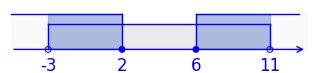
\includegraphics[width=0.3\textwidth]{fig_8.jpg}
    \end{center}

    \vspace{20pt}                            % dodaje 20 punktów odstępu w pionie
    \noindent
    \emph{\textbf{Odpowiedź:}}

    Rozwiązaniem nierówności $2 \leq |4 - x| < 7$ jest:
    \[x \in (-3, 2] \cup [6, 11)\]

    \vspace{150pt}                            % dodaje 20 punktów odstępu w pionie
    \noindent
    \begin{center}
    Wszystkie stworzone i wykorzystane w tym projekcie pliki oraz kod dostępne są na GitHub.
    \end{center}


\end{document}